%%%%%%%%%%%%%%%%%%%%%%%%%%%%%%%%%%%%%%%%%%%%%%%%%%%%%%%%%%%%%%%%%%%%%%%%%%%%%%%%
%2345678901234567890123456789012345678901234567890123456789012345678901234567890
%        1         2         3         4         5         6         7         8

\documentclass[letterpaper, 10 pt, conference]{ieeeconf}  % Comment this line out
                                                          % if you need a4paper
%\documentclass[a4paper, 10pt, conference]{ieeeconf}      % Use this line for a4
                                                          % paper

\IEEEoverridecommandlockouts                              % This command is only
                                                          % needed if you want to
                                                          % use the \thanks command
\overrideIEEEmargins
% See the \addtolength command later in the file to balance the column lengths
% on the last page of the document

% This is needed to prevent the style file preventing citations from linking to 
% the bibliography
\makeatletter
\let\NAT@parse\undefined
\makeatother

\usepackage[dvipsnames]{xcolor}

\newcommand*\linkcolours{ForestGreen}

\usepackage{times}
\usepackage{graphicx}
\usepackage{amssymb}
\usepackage{gensymb}
\usepackage{amsmath}
\usepackage{breakurl}
\def\UrlBreaks{\do\/\do-}
\usepackage{url,hyperref}
\hypersetup{
colorlinks,
linkcolor=\linkcolours,
citecolor=\linkcolours,
filecolor=\linkcolours,
urlcolor=\linkcolours}

\usepackage{algorithm}
\usepackage{algorithmic}

\usepackage[labelfont={bf},font=small]{caption}
\usepackage[none]{hyphenat}

\usepackage{mathtools, cuted}

\usepackage[noadjust, nobreak]{cite}
\def\citepunct{,\,} % Style file defaults to listing references separately

\usepackage{tabularx}
\usepackage{amsmath}

\usepackage{float}

\usepackage{pifont}% http://ctan.org/pkg/pifont
\newcommand{\cmark}{\ding{51}}%
\newcommand{\xmark}{\ding{55}}%

\newcommand*\diff{\mathop{}\!\mathrm{d}}
\newcommand*\Diff[1]{\mathop{}\!\mathrm{d^#1}}
\newcommand*\imgres{600}

\newcommand*\GitHubLoc{https://github.com/Jeffrey-Ede/ALRC}

\newcolumntype{Y}{>{\centering\arraybackslash}X}

%\usepackage{parskip}

\usepackage[]{placeins}

% \usepackage{epstopdf}
% \epstopdfDeclareGraphicsRule{.tif}{png}{.png}{convert #1 \OutputFile}
% \AppendGraphicsExtensions{.tif}

\newcommand\extraspace{3pt}

\usepackage{placeins}

\usepackage{tikz}
\newcommand*\circled[1]{\tikz[baseline=(char.base)]{
            \node[shape=circle,draw,inner sep=0.8pt] (char) {#1};}}
            
\usepackage[framemethod=tikz]{mdframed}

\usepackage{afterpage}

\usepackage{stfloats}

\usepackage{atbegshi}
\newcommand{\handlethispage}{}
\newcommand{\discardpagesfromhere}{\let\handlethispage\AtBeginShipoutDiscard}
\newcommand{\keeppagesfromhere}{\let\handlethispage\relax}
\AtBeginShipout{\handlethispage}

\usepackage{comment}

%\usepackage[1,2,3,5,6,7]{pagesel} %Discard page 4 as it is blank

% The following packages can be found on http:\\www.ctan.org
%\usepackage{graphics} % for pdf, bitmapped graphics files
%\usepackage{epsfig} % for postscript graphics files
%\usepackage{mathptmx} % assumes new font selection scheme installed
%\usepackage{times} % assumes new font selection scheme installed
%\usepackage{amsmath} % assumes amsmath package installed
%\usepackage{amssymb}  % assumes amsmath package installed

\title{\LARGE \bf
Predicting Hospital Re-admission in Diabetic Patients 
}

%\author{ \parbox{3 in}{\centering Huibert Kwakernaak*
%         \thanks{*Use the $\backslash$thanks command to put information here}\\
%         Faculty of Electrical Engineering, Mathematics and Computer Science\\
%         University of Twente\\
%         7500 AE Enschede, The Netherlands\\
%         {\tt\small h.kwakernaak@autsubmit.com}}
%         \hspace*{ 0.5 in}
%         \parbox{3 in}{ \centering Pradeep Misra**
%         \thanks{**The footnote marks may be inserted manually}\\
%        Department of Electrical Engineering \\
%         Wright State University\\
%         Dayton, OH 45435, USA\\
%         {\tt\small pmisra@cs.wright.edu}}
%}

\author{Crystal Chen$^{1}$ and Sara Golestaneh$^{2}$% <-this % stops a space
\thanks{$^{1}$Crystal is a MSc student in Statistics, 
University of Toronto, 
Email: chy.chen@mail.utoronto.ca}%
\thanks{$^{2}$Sara is a MSc student in Applied Computing, 
University of Toronto,
Email: sara.golestaneh@mail.utoronto.ca}%
}

% \author{Jeffrey M. Ede$^{1}$ and Richard Beanland$^{2}$% <-this % stops a space
% \thanks{*This work was not supported by any organization}% <-this % stops a space
% \thanks{$^{1}$H. Kwakernaak is with Faculty of Electrical Engineering, Mathematics and Computer Science,
%         University of Twente, 7500 AE Enschede, The Netherlands
%         {\tt\small h.kwakernaak at papercept.net}}%
% \thanks{$^{2}$P. Misra is with the Department of Electrical Engineering, Wright State University,
%         Dayton, OH 45435, USA
%         {\tt\small p.misra at ieee.org}}%
% }


\begin{document}


\maketitle
\thispagestyle{empty}
\pagestyle{empty}


%%%%%%%%%%%%%%%%%%%%%%%%%%%%%%%%%%%%%%%%%%%%%%%%%%%%%%%%%%%%%%%%%%%%%%%%%%%%%%%%
\begin{abstract}

Hospital re-admissions can be a drain on hospital resources, both in terms of time and money. As such, many in the healthcare industry are interested in reducing readmission rate to reap the numerous benefits. This project studied the factors which had the most significant impact on predicting hospital re-admission in patients with diabetes using a variety of binary classification methods. 

\end{abstract}

%%%%%%%%%%%%%%%%%%%%%%%%%%%%%%%%%%%%%%%%%%%%%%%%%%%%%%%%%%%%%%%%%%%%%%%%%%%%%%%%
\section{INTRODUCTION}

Hospital re-admissions can be caused by many factors from inadequate coordination by administrators\cite{medpac2007} to insufficient post-discharge care\cite{heartfailure}. Regardless of the reason, re-admission can have a negative impact on patients as their health issues may have progressed to a more serious stage compared to their previous visit, putting their life at greater risk. Furthermore, re-admissions increase costs as hospitals must allocate more resources to address cases which has been previously addressed. Lastly, re-admissions place further burdens upon healthcare workers as these re-admissions contribute to overcrowding which many hospitals already face. As such, it is not surprising that there is great interest in identifying factors which contribute to re-admission. 

In this project, the objective was to use binary classification to identify significant factors that predict re-admission in patients with diabetes. The data used was from the data set \textit{Diabetes 130 US Hospitals for years 1999 - 2008}. As the title implies, this publicly available dataset involved 130 American hospitals and recorded information regarding diabetic patients and their stay, ranging from their age and race, to their length of stay, the diagnoses and the kinds of medication they were prescribed. Note that as per similar research, only re-admissions under 30 days were considered\cite{survey}. Re-admissions over 30 days were not considered to be re-admissions.

%%%%%%%%%%%%%%%%%%%%%%%%%%%%%%%%%%%%%%%%%%%%%%%%%%%%%%%%%%%%%%%%%%%%%%%%%%%%%%%%
\section{Methods}

\subsection{Data Cleaning}

This dataset contained in total fifty variables in a variety of formats. First, ten highly problematic variables were removed. 

\begin{itemize}
    \item \textbf{Weight:} in the original dataset, approximately 97\% of patients were not weighed. As such, this variable was dropped as it was unlikely to be informative. 
    \item \textbf{Certain medication variables:} in general, there were 23 medication variables which indicated whether the patient was described the medication and/or whether their dosage had changed. However, nine of these features were removed as they fell into one of two categories - either the medication was never prescribed to any patients or the medication was prescribed to fewer than 100 patients. In either case, these features were so biased towards one level that they were not expected to have any explanatory power. The specific medications that were removed were acetohexamide, tolbutamide, troglitazone, examide, citoglipton, glipizide metformin, glimepiride pioglitazone, metformin rosiglitazone, and  metformin pioglitazone. 
\end{itemize}

Note that there were other variables which were missing 30-50\% of their values (e.g. A1C results and Payer Code). However, these were deemed likely to still have some explanatory power and so, did not warrant removal. Furthermore, A1C results had been shown to be significant for predicting re-admission. As such, only features that were missing over 95\% of its data were removed. 

Secondly, any patients who had a disposition ID of 11, 13, 14, 19-21 were removed. These patients either passed away or were transferred to a hospice and as such, were unlikely to ever be readmitted\cite{ref1}\cite{ref2}. Given the target population are patients who have a possibility of being readmitted, these patients were removed as they did not fit that criterion. 

Lastly, the remaining variables were processed depending on their type. The remaining numerical variables required no processing because there appeared to be no instances of missing or erroneous  values. One notable change is Age which was originally an ordinal variable with patient's age being indicated by a range (e.g. 0-9, 10-19, etc.). This was transformed into a numerical variable by taking the midpoint of each age range as an estimate of patients' age. Converting Age into a numerical variable makes more sense as it is just more common to treat age as a numeric value. 

For the remaining categorical variables, any missing/unknown values were grouped into an "Unknown"/"Other" category. Then, they all received the one-hot encoding where each level in a feature becomes its own indicator function. Note however that features such as Diagnosis 1-3 and Medical Specialty contains many levels (e.g. Diagnosis 1 contains 718 levels). As such, if all levels became an indicator function, then overfitting may be an issue in modelling. These particular variables were reduced to only eleven levels where only the top ten most frequent labels were retained and all other labels were relabelled as "Other". 

\subsection{Exploratory Data Analysis}

The motivation behind the exploratory data analysis (EDA) was to investigate features which were intuitively linked to health; if a patient was experiencing more severe health issues, they may be more likely to be re-admitted. There was also interest in identifying whether certain groups of people were more likely to be readmitted. This analysis was completed through a series of visualizations (i.e. pie charts, stacked bar graphs and box plots) often relating features of interest to rate of re-admission. 

\subsection{Balancing out the Data}
One of the major problems with this data set that needed to be resolved before modeling, was that the data was highly imbalanced. More specifically, the number of the patients who were readmitted within 30 days was much lower than the number of the patients who were not readmitted (see Fig.~\ref{imb}).\\

\begin{figure}[!hbt]
\centering
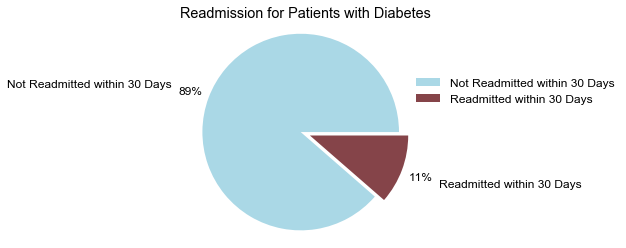
\includegraphics[width=1\columnwidth]{imbalanced.png}
\caption{Proportion of readmitted patients vs. non-readmitted patients}
\label{imb}
\end{figure}\\

As seen in Fig.~\ref{imb}, readmitted patients only cover up around 11$\%$ of all patients. Since the main goal of this project was to correctly classify the patients that were readmitted, not having enough data about this group could pose a problem and could cause models to be highly biased. To address this issue, there are two main solutions:

\subsubsection{Undersampling the Majority Class} The main way to to do this is by randomly choosing a subset of data in the majority class (also called "Random Undersampling"). This results in a balanced but smaller version of the original data set.

\subsubsection{Oversampling the Minority Class}
There are two main ways to implement oversampling. One way is to simply choose a random subset of the minority class and then duplicate it to populate the dataset and create classes of equal size. The other method is to synthesise a new dataset through SMOTE (Synthetic Minority Oversampling Technique). Random oversampling and undersampling were initially used in this project. However since random oversampling behaved similarly to random undersampling, focus was shifted to comparing random undersampling and SMOTE oversampling method.

\subsection{Modelling}
This project focused on applying and comparing three different tree-based models:

\subsubsection{Random Forest}
A random forest is a meta estimator that fits a number of decision tree classifiers on various sub-samples of the dataset and uses averaging to improve the predictive accuracy and control over-fitting.

\subsubsection{Gradient Boosting}
Gradient Boosting builds an additive model in a forward stage-wise fashion and allows for the optimization of arbitrary differentiable loss functions. In each stage, regression trees are fitted on the negative gradient of the binomial or multinomial deviance loss function. Since this is a binary classification, only a single regression tree is induced in each stage.

\subsubsection{XGBoost} 
XGBoost (Extreme Gradient Boosting) is similar to normal gradient boosting with a few optimizations. While regular gradient boosting uses the loss function of the base model (e.g. decision tree) as a proxy for minimizing the error of the overall model, XGBoost uses the 2nd order derivative as an approximation. Also, xgboost uses a more regularized model formalization to control over-fitting, which gives it better performance.\\\\

Please note that since there were no timestamps associated with the data points in the dataset, they could not be treated as time series data. On the other hand, since multiple rows could belong to one patient visiting the hospital on different days, the data points were not completely independent. For such data, tree-based models are the best, since they do not make any strict assumption about the independence of the data (unlike logistic regression).

\subsection{Cross-Validation}
To evaluate the models and compare the results from using oversampling and undersampling, a 5-fold stratified cross validation was used. When doing cross validation along with balancing out techniques, undersampling and oversampling were only applied on the training partitions and the validation partition would remain untouched.

\subsection{Hyper-parameter Tuning}
After choosing the best model based on different metrics (especially recall and AUC), 2-fold cross-validation was applied along with a grid search on possible parameters to do the hyper-parameter tuning. The grid search was completed over the following parameters: learning rate: [0.001,0.01,0.1], maximum depth: [1,3,5,7,9] and number of estimators (decision trees): [100,200,\dots,500]. The metric that was optimized at this stage was AUC.

\subsection{Feature Importance and SHAP values}
To interpret the final model, SHAP values were used. SHAP or SHapley Additive exPlanations is a game theoretic approach that is used on tree-based models to compute the contribution of each feature to the predictions. It connects optimal credit allocation with local explanations using the classic Shapley values from game theory and their related extensions \cite{GitHub}. 

%%%%%%%%%%%%%%%%%%%%%%%%%%%%%%%%%%%%%%%%%%%%%%%%%%%%%%%%%%%%%%%%%%%%%%%%%%%%%%%%
\section{Results}

\subsection{Exploratory Data Analysis}

There are a few important observations to note from the EDA. The main observation is that the dataset is unbalanced in a variety of manners. Recall, there are far fewer readmitted patients (approx. 11.4\%) compared to non-readmitted ones (see Fig.~\ref{imb}). This is to be expected as re-admissions are not so high that the proportion of readmitted patients is comparable to non-readmitted patients. This dataset is also unbalanced in terms of race and gender. Approximately 75\% of patients are Caucasian with the second largest racial group being African Americans (19\%) (see Fig.~\ref{race} in Appendix). However, proportion of readmitted patients within each group is relatively constant at around 10-11\% (see Fig.~\ref{raceprop} in Appendix). Similarly, the population is made up of 53\% females and 37\% males, with re-admission rates among the two groups being almost the same (11.5\% vs. 11.3\% respectively) (see Fig.~\ref{gender} in Appendix). 

\begin{figure}[!hbt]
\centering
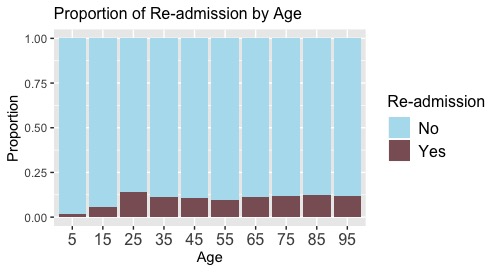
\includegraphics[width=1\columnwidth]{Rplot.png}
\caption{Proportion of readmitted patients vs. non-readmitted patients for each age group}
\label{ageprop}
\end{figure}\\

A majority of patients were also in the 50-89 age range (see Fig.~\ref{age} in Appendix), which is unsurprising given that older people are more likely to experience health problems and so, visit the hospital more. Unexpectedly however, re-admission rates peak in the 20-29 age group and remain relatively stable for patients aged 30-99 (see Fig.~\ref{ageprop}). One would expect patients who are more likely to experience more severe health issues at a higher frequency (i.e. older patients) to be readmitted more than younger, healthier patients. Keeping in mind that this dataset involves diabetic patients, one potential explanation is that patients aged 20-29 are likely beginning to live independently and are at an age where they are still somewhat inexperienced with managing their illness. Thus, they may be readmitted more often compared to older patients who have more experience and even younger patients who are cared for by their parents.  

It also appears that particular diagnoses are prone to higher rates of re-admission compared to others. The proportion of readmitted patients under and over 30 days vs. non-readmitted patients for the first, second and third diagnoses can be observed in Fig.~\ref{diag1}, ~\ref{diag2} and ~\ref{diag3} respectively. 

In the first diagnosis, the top three outcomes with the highest re-admission rates are, in decreasing order, heart failure (ID: 428), chronic bronchitis (ID: 491) and acute myocardial infarction (ID: 410). In the second diagnosis, the top three outcomes are hypertension renal disease (ID: 403),  disorders of fluid, electrolytes and acid-balance (ID: 276) and once again, heart failure. In the third diagnosis, hypertension renal disease and fluid, electrolytes and acid-balance disorders were once again among the top three outcomes with the highest re-admission along with chronic renal failure (ID: 585). Based on these observations, heart failure, hypertension renal disease and disorders of fluid, electrolytes and acid-balance are conditions that doctors should possibly pay closer attention to as they are not only some of the most frequent diagnoses and have the highest re-admission rates, but also appear multiple times in different diagnoses. As an aside, the "Other" outcome in all three diagnoses have high re-admission rates, but recall that any outcome that was not one of the ten most frequent diagnoses were collapsed into this category. As such, the category contains too wide range of diagnoses to make any concrete observations about it. 

\begin{figure}[!hbt]
\centering
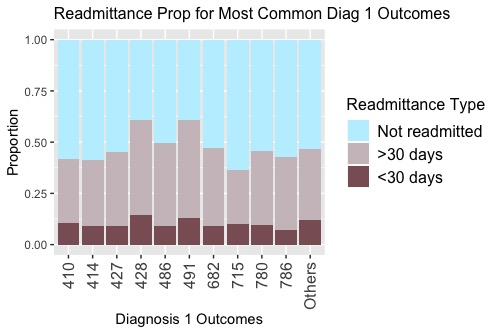
\includegraphics[width=1\columnwidth]{Rplot01.png}
\caption{Proportion of readmitted patients over and under 30 days vs. non-readmitted patients for top 10 most common outcomes of first diagnosis}
\label{diag1}
\end{figure}

\begin{figure}[!hbt]
\centering
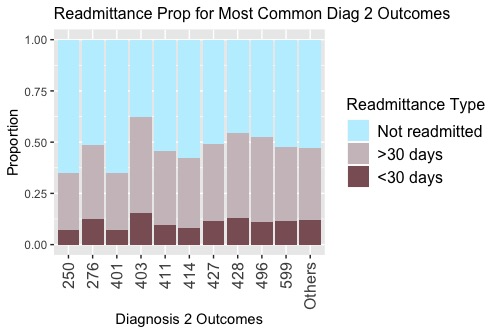
\includegraphics[width=1\columnwidth]{Rplot02.png}
\caption{Proportion of readmitted patients over and under 30 days vs. non-readmitted patients for top 10 most common outcomes of second diagnosis}
\label{diag2}
\end{figure}

\begin{figure}[!hbt]
\centering
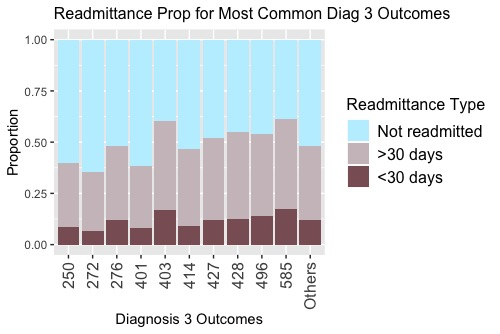
\includegraphics[width=1\columnwidth]{Rplot03.png}
\caption{Proportion of readmitted patients over and under 30 days vs. non-readmitted patients for top 10 most common outcomes of third diagnosis}
\label{diag3}
\end{figure}\\

Lastly, the distributions of the number of medications that patients regularly take as well as the total number of procedures they undergo (whether be it lab tests or other procedures) did not seem to differ between patients who were readmitted and patients who were not readmitted. This indicates that these features likely will not play a significant role in predicting whether or not a patient is readmitted. 

 To reproduce the results of this section, see the EDA Rmarkdown file.

\subsection{Model Results Using Random Undersampling and SMOTE}
After evaluating the models using 5-fold cross-validation, it was observed that SMOTE resulted in higher accuracy in general. The difference in the accuracies can be seen in Table ~\ref{tab:accs}  evaluated using cross-validation (Also see Fig.~\ref{rusbp} and Fig.~\ref{osbp} in Appendix). \\
	        	\begin{table}[!hbt]
		% Center the table
		\begin{center}

\begin{tabular*}{\columnwidth}{@{\extracolsep{\fill}}c|ccc}

\hline
\multicolumn{1}{c|}{}       & \multicolumn{2}{c}{Random Undersample} & \multicolumn{1}{c}{SMOTE}  \\
Model Name         & \multicolumn{2}{c}{Mean accuracy} & \multicolumn{1}{c}{Mean accuracy}         \\ \hline
Random Forest &  & 0.615 & 0.735 \\
Gradient Boosting &   & 0.651 & 0.884 \\
XGBoost &  & 0.652 & 0.884  \\

\hline
\end{tabular*}
		\caption{Random Undersampling vs SMOTE Results Using Cross-validation}
		\label{tab:accs}
		\end{center}
	\end{table}\\
 Although it seems like SMOTE results in higher accuracy, other metrics such as the recall of the positive class is more important for the purposes of this project. Table ~\ref{tab:metrics} shows the difference in accuracy, recall for the positive class and AUC metrics between the two methods when models were evaluated on the test set.
	        	\begin{table}[!hbt]
		% Center the table
		\begin{center}

\begin{tabular*}{\columnwidth}{@{\extracolsep{\fill}}c|ccc|ccc}

\hline
\multicolumn{1}{c|}{}       & \multicolumn{3}{c}{Random Undersample} & \multicolumn{3}{c}{SMOTE}  \\
Model Name         & \multicolumn{1}{c}{Recall} & Acc& AUC&

\multicolumn{1}{c}{Recall} & Acc & AUC        \\ \hline
Random Forest & 0.63  & 0.61& 0.615&0.34&0.74&0.565 \\
Gradient Boosting &0.59  & 0.65 & 0.620  &0.03&0.89&0.510\\
XGBoost & 0.59  & 0.65 & 0.623& 0.03&0.89&0.509\\

\hline
\end{tabular*}
		\caption{Random Undersampling vs SMOTE: AUC and Recall of Readmitted patients evaluated on Test set}
		\label{tab:metrics}
		\end{center}
	\end{table}
 Unfortunately, SMOTE resulted in much lower recall and AUC compared to random undersampling. In other words, when SMOTE was used to balance the dataset, models became more conservative and labeled as few positive cases as possible, resulting in lower recall but higher accuracy. As mentioned, since both higher AUC and higher accuracy along with good recalls for positive class are more important for this project, XGBoost with random undersampling was chosen as producing the best results (since the AUC is a little bit higher compared to other models).\\
 The best parameters resulted from the grid search were: learning rate: 0.1, maximum depth:3 and number of estimators: 100, which is by coincidence the same default parameters that we used to train our model.\\
 Fig.~\ref{confusion} shows the confusion matrix of the best model. As we can see the main reason behind the low accuracy is the high number of false positives.\\

 \begin{figure}[!hbt]
\centering
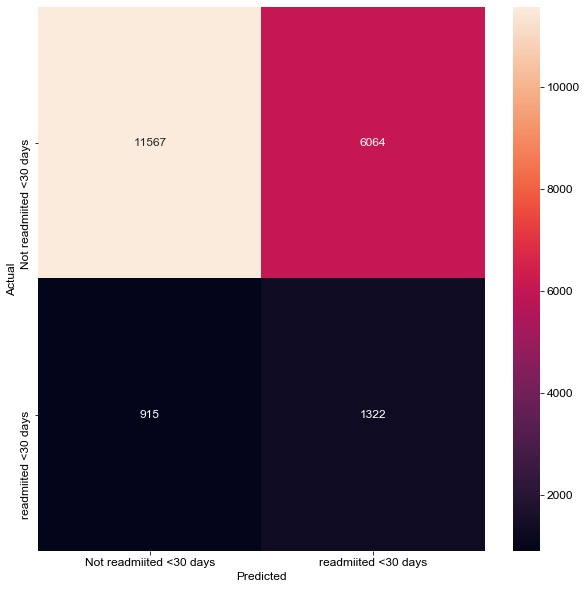
\includegraphics[width=0.9\columnwidth]{cmbest.png}
\caption{XGBoost Confusion Matrix on the Test set}
\label{confusion}
\end{figure}
 To reproduce the results of this section, run the Undersample notebook. For SMOTE results, run the Oversample notebook.
 \subsection{SHAP Feature Importance Results}
 Fig.~\ref{shapfeatures} shows the top 20 features based on the shap values.
 \begin{figure}[!hbt]
\centering
\textbf{XGBoost Top Features}\par\medskip
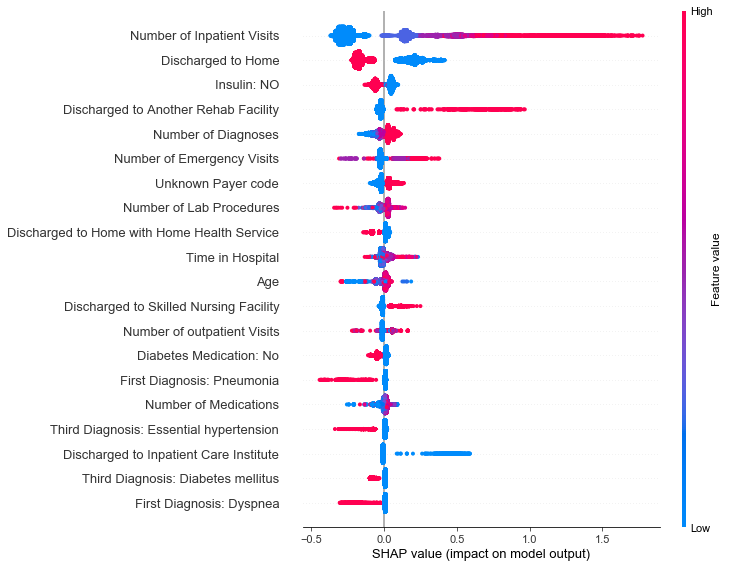
\includegraphics[width=1\columnwidth]{shapfeatures.png}
\caption{Top 20 Features of the XGBoost Model Based on SHAP values. Every patient has one dot on each row. The x position of the dot is the impact of that feature on the model’s prediction for the patient, and the color of the dot represents the value of that feature for the patient. Dots that don’t fit on the row pile up to show density. Since the XGBoost model has a logistic loss the x-axis has units of log-odds (Tree SHAP explains the change in the margin output of the model)}
\label{shapfeatures}
\end{figure}\\

As shown in the graph above, some of the features such as the number of inpatient visits in the year preceding the encounter or being discharged to another rehab facility have a positive affect on being readmitted within 30 days. In other words if the patient has had a higher number of inpatient visits or if they were transferred to another rehab facility, there is higher probability that they will be readmitted within 30 days. Features such as being discharged to home, no insulin and no diabetes medication have a negative effect on the prediction, meaning if the patient is discharged to home or if they were not prescribed any insulin (or any diabetes medication), there is higher chance that they will not get readmitted within 30 days. Furthermore, the higher the number of diagnoses, the higher the chance of being readmitted within 30 days (based on the model). Older patients and patients that spent a longer time in the hospital are more likely to be readmitted within 30 days. Two final interesting observations are that if the patient is diagnosed with pneumonia or dyspnea (a breathing problem) as the first diagnosis or essential hypertension or diabetes mellitus as the third diagnosis, there will be a lower probability of getting readmitted within 30 days.\\

To reproduce the results of this section, see the Undersample notebook, SHAP Values section.

%%%%%%%%%%%%%%%%%%%%%%%%%%%%%%%%%%%%%%%%%%%%%%%%%%%%%%%%%%%%%%%%%%%%%%%%%%%%%%%%
\section{Discussion & Conclusion}

Overall, this project revealed both surprising and unsurprising results. Through EDA, it was observed that features such as gender and race likely do not play a major role in predicting re-admission given the similar rates between groups. Similar conclusions were made regarding number of medications that patients take as well as the total number of procedures they undergo during their visit. It was surprising to see that while the majority of patients were over 50, 20-29 year olds experienced the highest re-admission rate. This could possibly be due to the new-found independence that patients in this age group experience and the lack of experience they have with managing diabetes. Lastly, it was noted that diagnoses such as hypertension renal disease, heart failure and disorders of fluid, electrolytes and acid balance were common conditions that had high re-admission rates. 

However, the results of modelling notes that the most significant factors which predict re-admission are a combination of both the patient's patterns of behaviour (e.g. number of emergency visits and number of inpatient visits) and particular outcomes of their visit (e.g. discharged to home/another rehab/nursing facility) and the condition of their wellness which is somewhat indicated by whether they were prescribed insulin or any diabetes medication or not. Also, the models attributes higher rate of re-admission to older ages which is not necessary true.

\section{Future Considerations}

There are a few final considerations to be noted for this project. Firstly, as with all data analysis, preprocessing is key. In this project, the number of categories in diagnosis and medical specialty were reduced by keeping only the top ten most frequent diagnoses/specialties and re-categorizing all others as "Other". While this is a reasonable way to reduce the number of features, this method is limited to only interpretations regarding specific diseases. Alternatively,  medical classes could have been used to reduce the number of categories. For example, the diagnoses could be classified into their ICD 9 classes (e.g. diseases of circulatory system, nervous system, respiratory system, etc.). This would have allowed for more general interpretations of the results. Secondly, only one type of oversampling and undersampling was investigated. Many other oversampling methods (e.g. SVMSMOTE) or undersampling methods (e.g. Condensed Nearest Neighbours) or even a combination of those could potentially result in higher AUC or recalls. Lastly, calibrating the models could potentially produce better results.

%%%%%%%%%%%%%%%%%%%%%%%%%%%%%%%%%%%%%%%%%%%%%%%%%%%%%%%%%%%%%%%%%%%%%%%%%%%%%%%%

\bibliographystyle{ieeetr}
\bibliography{bibliography}
\newpage
\section{Appendix}

\begin{figure}[!hbt]
\centering
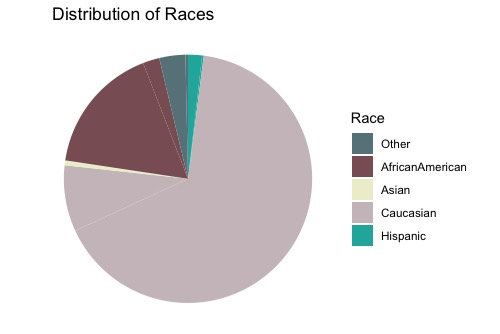
\includegraphics[width=1\columnwidth]{Rplot04.png}
\caption{Distribution of races}
\label{race}
\end{figure}\\

\begin{figure}[!hbt]
\centering
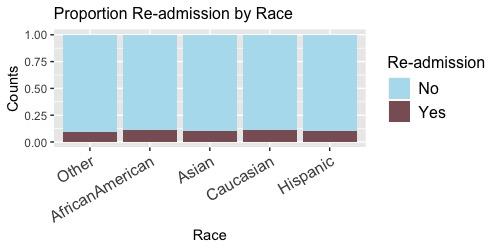
\includegraphics[width=1\columnwidth]{Rplot05.png}
\caption{Proportion of readmitted patients in each race}
\label{raceprop}
\end{figure}\\

\begin{figure}[!hbt]
\centering
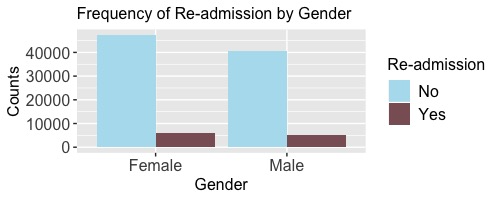
\includegraphics[width=1\columnwidth]{Rplot06.png}
\caption{Frequency of readmitted patients vs. non-readmitted patients for various genders}
\label{gender}
\end{figure}\\

\begin{figure}[!hbt]
\centering
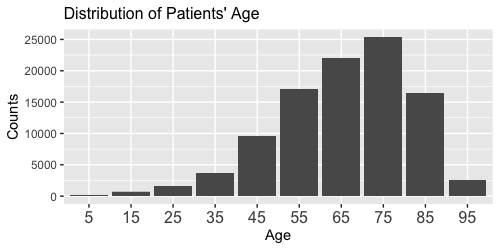
\includegraphics[width=1\columnwidth]{Rplot07.png}
\caption{Number of patients in each age group}
\label{age}
\end{figure}\\

\begin{figure}[!hbt]
\centering
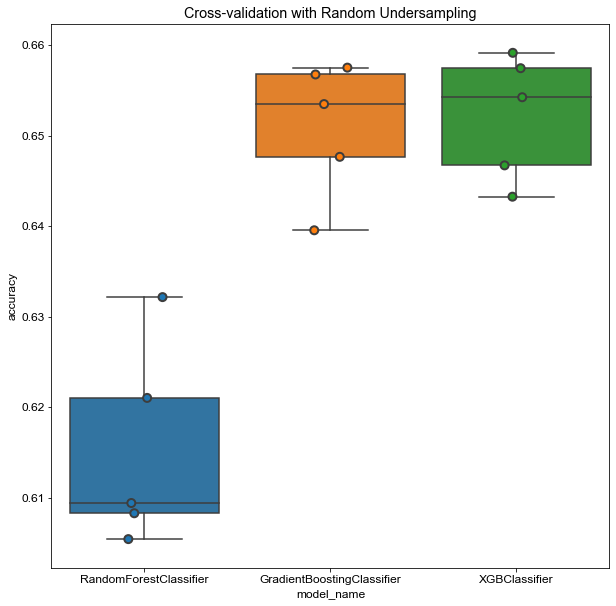
\includegraphics[width=1\columnwidth]{rusbp.png}
\caption{Boxplot of accuracies of three models using Random undersampling and 5-fold cross-validation}
\label{rusbp}
\end{figure}

\begin{figure}[!hbt]
\centering
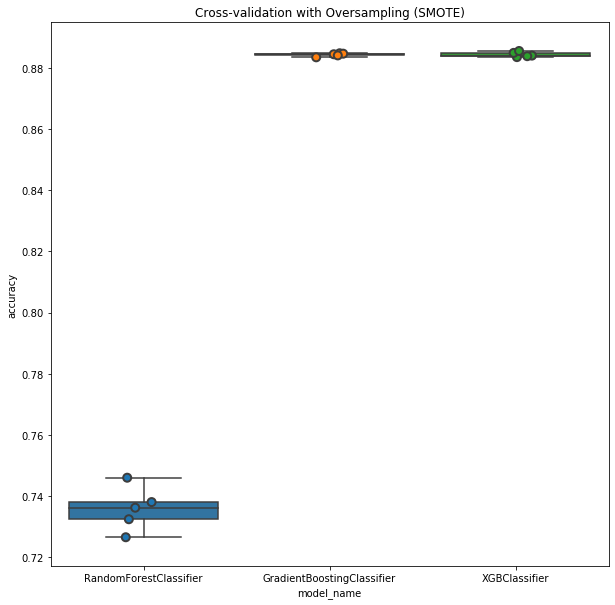
\includegraphics[width=1\columnwidth]{smotebp.png}
\caption{Boxplot of accuracies of three models using SMOTE (oversampling) and 5-fold cross-validation}
\label{osbp}
\end{figure}
\clearpage

\end{document}
